% Source: fixed 2006 Zhejiang science scan, PDF page 1, Q9.
% Schematic projection; retain the three mutually perpendicular radii and
% the arc-midpoint labels on the great-circle arcs AB and AC.
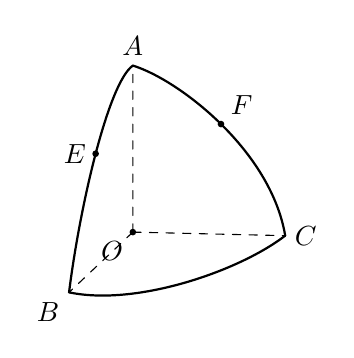
\begin{tikzpicture}[line cap=round,line join=round,x=0.9cm,y=0.9cm]
  \coordinate (O) at (0,0);
  \coordinate (A) at (0,2.35);
  \coordinate (B) at (-0.9,-0.85);
  \coordinate (C) at (2.15,-0.05);
  % Parameter midpoints of the two schematic cubic Bezier arcs.
  \coordinate (E) at (-0.525,1.10625);
  \coordinate (F) at (1.24375,1.525);
  % Schematic visible spherical boundary and the two great-circle arcs.
  \draw[thick] (A) .. controls (-0.35,2.1) and (-0.75,0.35) .. (B);
  \draw[thick] (A) .. controls (0.65,2.15) and (1.95,1.15) .. (C);
  \draw[thick] (B) .. controls (0.05,-1.05) and (1.5,-0.55) .. (C);
  \draw[dashed] (O)--(A) (O)--(B) (O)--(C);
  \fill (O) circle (1.2pt) (E) circle (1.2pt) (F) circle (1.2pt);
  \node[above] at (A) {$A$};
  \node[below left] at (B) {$B$};
  \node[right] at (C) {$C$};
  \node[below left] at (O) {$O$};
  \node[left] at (E) {$E$};
  \node[above right] at (F) {$F$};
\end{tikzpicture}
